\chapter{傅立叶级数}
\section{波的时域与空域}
当谈到频率的时候,一定假定主体是一个周期信号,这意味着信号的时间是从负无穷持续到正无穷,这时时间就不再是一个变量。

For example, you stand at a fixed point in the ocean (or on an electrical circuit) and the waves (or the electrical current) wash over you with a regular, recurring pattern of crests and troughs. The height of the wave is a periodic function of time. Sound is another example: “sound” reaches your ear as a longitudinal pressure wave, a periodic compression and rarefaction of the air. In the case of space, you come to the phenomenon. You take a picture and you observe repeating patterns.
\begin{enumerate}
	\item 空间固定,使用频率表示一秒内经过多少个波;
	\item 时间固定,使用周期描述波在空间上的分布;
	\item 时域上用频率表示周期性;空域上用周期表示周期性。周期和频率互成反比:
	      \begin{align*}
		       & \lambda  & = & v     & \cdot   \quad & \frac{1}{\theta} \\
		       & Distance & = & Speed & \times  \quad & Time
	      \end{align*}
\end{enumerate}

\section{信号周期化}
\subsection{笔记中周期的设定}
\begin{enumerate}
	\item 在下面的笔记里,我们一直设定周期为$1$,即:
	      \begin{equation}
		      f(t+1)=f(t)
	      \end{equation}
	\item 周期为$1$的信号,可以用$sin(2\cdot \pi \cdot t)$和$cos(2\cdot \pi \cdot t)$组成。

\end{enumerate}
\subsection{为什么用三角函数表示周期性}
三角函数作为线性系统的输入时具有频率不变的特性。

假设输入信号为$x(t)=\cos (\omega\cdot t)$。输出信号为输入信号$\cos (\omega\cdot t)$加上一个时延信号$\alpha\cdot \cos (\omega\cdot t-\omega\cdot t_0)$:
\begin{align*}
	  & g(t)                                                            \\
	= & \cos(w\cdot t)+\alpha\cdot \cos (\omega\cdot t-\omega\cdot t_0) \\
	= & (1+\alpha \cdot \cos\omega\cdot t_0)\cdot \cos (\omega\cdot t)  \\
	+ & \alpha\cdot \sin(\omega\cdot t_0)\cdot \sin(\omega\cdot t)      \\
	= & A\cdot \cos(\omega\cdot t-\theta)
\end{align*}

从这个例子可以看出,输入是一个余弦信号,输出也是一个余弦信号。只是幅度和相位有了一定改变,但是频率没有变。
\subsection{One period, many frequencies.}
Is the sum of two periodic functions periodic?
\begin{figure}[H]
	\centering
	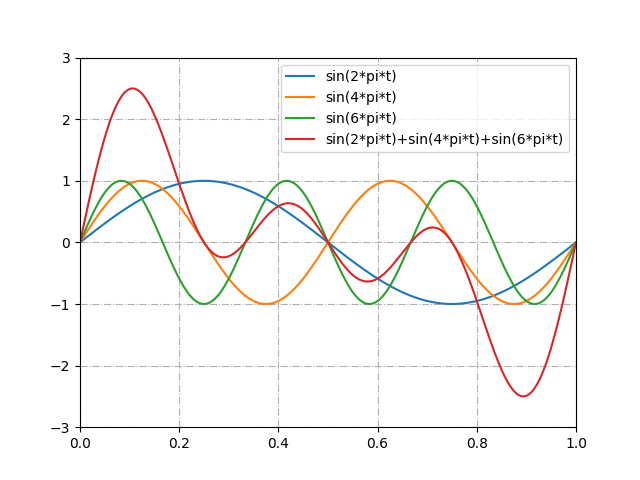
\includegraphics[width=0.4\textwidth]{assets/Figure_1.png}
	\caption{$\sin(2\cdot\pi\cdot t)+\sin(4\cdot\pi\cdot t)+\sin(8\cdot\pi\cdot t)$}
\end{figure}
\begin{enumerate}
	\item 一般表示为:
	      \begin{equation}\label{vtri}
		      f(t)=\sum\limits_{k=1}^n\ A_k\cdot \sin(2\cdot \pi\cdot k\cdot t+\phi_k)
	      \end{equation}
	      This form of a general trigonometric sum has the advantage of displaying explicitly the amplitude and phase of each harmonic, but it turns out to be somewhat awkward to calculate with.

	      这里使用$\cos$也没有关系,但是这节课里就钦定了$\sin$。
	\item 由上图可以看出,整体的函数在周期最长的函数重复的时候才重复,可以说周期最长的函数奠定了整个函数的基调。$k=1​$时,$T=\frac{2\cdot \pi}{2\cdot \pi}=1​$,周期最长,所以$k=1​$的项被称为fundamental wave。而$k>1​$的项被称为harmonic wave。
\end{enumerate}

\section{傅立叶级数的两种表达方式}
\subsection{三角函数形式表示}
我们把\ref{vtri}展开:
\begin{align*}
	      & f(t)                                                                                                   \\
	=     & \sum\limits_{k=1}^n\ A_k\cdot \sin(2\cdot\pi\cdot k\cdot t+\phi_k)                                     \\
	=     & \sum\limits_{k=1}^n\ [A_k\cdot \sin(2\cdot\pi\cdot k\cdot t)                                           \\
	\cdot & \cos(\phi_k)+A_k\cdot \cos(2\cdot \pi\cdot k\cdot t)\cdot \sin(\phi_k)]                                \\
	=     & \sum\limits_{k=1}^n\ [a_k\cdot \sin(2\cdot\pi\cdot k\cdot t) +b_k\cdot \cos(2\cdot \pi\cdot k\cdot t)]
\end{align*}

其中:
$$
	\left\{
	\begin{array}{lr}
		a_k=A_k\cdot \cos(\phi_k) \\
		b_k=A_k\cdot \sin(\phi_k)
	\end{array}
	\right.
$$

所以我们得到:
\begin{equation}
	f(t) =\sum\limits_{k=1}^n\ [a_k\cdot \sin(2\cdot\pi\cdot k\cdot t) +b_k\cdot \cos(2\cdot \pi\cdot k\cdot t)]
\end{equation}

我们还可以给它加一个直流分量$\frac{A_0}{2}$:
\begin{equation}\label{vtrii}
	f(t) =\sum\limits_{k=1}^n\ [a_k\cdot \sin(2\cdot\pi\cdot k\cdot t) +b_k\cdot \cos(2\cdot \pi\cdot k\cdot t)]+\frac{A_0}{2}
\end{equation}

这里为啥直流分量取$\frac{A_0}{2}$后面会说。
\subsection{复指形式表示}
因为根据\eqref{vtrii}的展开,所以我们令(为什么这么令我也不知道,反正老师就是突然跳到这一步。他想怎么干就怎么干吧……):
\begin{equation}
	f(t)=\sum\limits_{k=-n}^n\ c_k\cdot e^{2\cdot \pi \cdot i \cdot k \cdot t}
\end{equation}

注意到,当$k=0$时,$f(t)=\frac{A_0}{2}=c_0=\overline{c_0}$。
\section{欧拉公式}
\begin{equation}
	e^{2\cdot \pi\cdot i\cdot k\cdot t} =  \cos(2\cdot \pi\cdot k\cdot t)+i\cdot \sin(2\cdot \pi\cdot k\cdot t)
\end{equation}
\begin{equation}
	\cos(2\cdot \pi\cdot k\cdot t)=\frac{e^{2\cdot \pi\cdot i\cdot k\cdot t+}+e^{-2\cdot \pi\cdot i\cdot k\cdot t}}{2}
\end{equation}
\begin{equation}
	\sin(2\cdot \pi\cdot k\cdot t)=\frac{e^{2\cdot \pi\cdot i\cdot k\cdot t+}-e^{-2\cdot \pi\cdot i\cdot k\cdot t}}{2\cdot i}
\end{equation}
\section{傅立叶级数的对称性}

假设​信号是一个实信号(real 信号),则信号中没有虚部,有​$f(t)=\overline {f(t)}$:
\begin{align*}
	  & f(t)                                                                                        \\
	= & \sum\limits_{k=-n}^n\ c_k\cdot e^{2\cdot \pi \cdot i \cdot k \cdot t}                       \\
	= & \overline{\sum\limits_{k=-n}^n\ c_k\cdot e^{2\cdot \pi \cdot i \cdot k \cdot t}}            \\
	= & \sum\limits_{k=-n}^n\ \overline{c_k}\cdot \overline{e^{2\cdot \pi \cdot i \cdot k \cdot t}} \\
	= & \sum\limits_{k=-n}^n\ \overline{c_k}\cdot e^{-2\cdot \pi \cdot i \cdot k \cdot t}
\end{align*}

因为$\sum\limits_{k=-n}^n=\sum\limits_{k=n}^{-n}$,所以把$k$变成$-k$,得:
\begin{align*}
	  & f(t)                                                                        \\
	= & \sum\limits_{k=-n}^n\ c_k\cdot e^{2\cdot \pi \cdot i \cdot k \cdot t}       \\
	= & \sum\limits_{-k=-n}^n\ c_{-k}\cdot e^{2\cdot \pi \cdot i \cdot k \cdot t}   \\
	= & \sum\limits_{k=n}^{-n}\ c_{-k}\cdot e^{-2\cdot \pi \cdot i \cdot k \cdot t} \\
	= & \sum\limits_{k=-n}^n\ c_{-k}\cdot e^{-2\cdot \pi \cdot i \cdot k \cdot t}
\end{align*}

由上面两个推导知:
$$
	f(x)=\sum\limits_{k=-n}^n \overline{c_k}\cdot e^{-2\cdot \pi \cdot i \cdot k \cdot t}=\sum\limits_{k=-n}^n c_{-k}\cdot e^{-2\cdot \pi \cdot i \cdot k \cdot t}
$$


所以得到:
\begin{equation}
	c_{-k}=\overline{c_k}
\end{equation}

那么我们可知:
\begin{align*}
	  & c_k\cdot e^{2\cdot \pi\cdot i\cdot k\cdot t}+c_{-k}\cdot e^{2\cdot \pi\cdot i\cdot (-k)\cdot t}                 \\
	= & c_k\cdot e^{2\cdot \pi\cdot i\cdot k\cdot t}+c_{-k}\cdot e^{-2\cdot \pi\cdot i\cdot k\cdot t}                   \\
	= & c_k\cdot e^{2\cdot \pi\cdot i\cdot k\cdot t}+\overline{c_k}\cdot e^{\overline{2\cdot \pi\cdot i\cdot k\cdot t}} \\
	= & c_k\cdot e^{2\cdot \pi\cdot i\cdot k\cdot t}+\overline{c_k\cdot e^{2\cdot \pi\cdot i\cdot k\cdot t}}            \\
	= & 2\cdot \Re\{C_k\cdot e^{2\cdot \pi \cdot i\cdot k\cdot t}\}
\end{align*}

所以$c_k\cdot e^{2\cdot \pi\cdot i\cdot k\cdot t}+c_{-k}\cdot e^{2\cdot \pi\cdot i\cdot (-k)\cdot t}$为一个实数。$\sum\limits_{k=-n}^n\ c_k\cdot e^{2\cdot \pi \cdot i \cdot k \cdot t}$可以表示一个实数。

\section{从三角函数到复指形}
\subsection{从三角函数到复指形}
\begin{align*}
	  & f(t)                                                                                                                      \\
	= & \sum\limits_{k=1}^n\ [a_k\cdot \sin(2\cdot\pi\cdot k\cdot t)                                                              \\
	+ & b_k\cdot \cos(2\cdot \pi\cdot k\cdot t)]+\frac{A_0}{2}                                                                    \\
	= & \sum\limits_{k=1}^n\ (a_k\cdot \frac{e^{2\cdot \pi\cdot i\cdot k\cdot t}- e^{-2\cdot \pi\cdot i\cdot k\cdot t}}{2\cdot i} \\
	+ & b_k\cdot \frac{e^{2\cdot \pi\cdot i\cdot k\cdot t+}+e^{-2\cdot \pi\cdot i\cdot k\cdot t}}{2})+\frac{A_0}{2}               \\
	= & \sum\limits_{k=1}^n\ (\frac{b_k-i\cdot a_k}{2}\cdot e^{2\cdot \pi\cdot i\cdot k\cdot t}                                   \\
	+ & \frac{b_k+i\cdot a_k}{2}\cdot e^{-2\cdot \pi\cdot i\cdot k\cdot t})+\frac{A_0}{2}
\end{align*}
设$c_0=\frac{1}{2}\cdot A_0$;$c_k=\frac{b_k-i\cdot a_k}{2}$;$c_{-k}=\overline{c_{k}}=\frac{b_k+i\cdot a_k}{2}$则:
\begin{align*}
	  & f(t)                                                                                                                          \\
	= & \sum\limits_{k=1}^n\ (c_k\cdot e^{2\cdot \pi\cdot k\cdot t}+c_{-k}\cdot e^{-2\cdot \pi\cdot k\cdot t})+c_0                    \\
	= & \sum\limits_{k=1}^n\ c_k\cdot e^{2\cdot \pi\cdot k\cdot t}+\sum\limits_{k=1}^n\ c_{-k}\cdot e^{-2\cdot \pi\cdot k\cdot t}+c_0 \\
	= & \sum\limits_{k=1}^n\ c_k\cdot e^{2\cdot \pi\cdot k\cdot t}+\sum\limits_{k=-1}^{-n}\ c_k\cdot e^{2\cdot \pi\cdot k\cdot t}+c_0 \\
	= & \sum\limits_{k=-n\ k\neq0}^n\ c_k\cdot e^{2\cdot \pi\cdot k\cdot t}+c_0
\end{align*}

为了表示一般的周期现象,光求$\sum\limits_{k=-n}^n$是不够的,我们必须考虑对周期信号进行无限项求和,即求:$\sum\limits_{k=-\infty}^\infty$。

We can use high frequencies to make sharp corners.
There is discontinuity in some high derivative that means that you are gonna have trouble repeating that phenomenon as a finite sum.
You are gonna have to make N layers and layers to represent it more and more accurately.

由于$\cos(x)$和$\sin(x)$是连续且无限可微分的,所以有限的$\cos(x)$或$\sin(x)$之和不能表示离散的函数或者不无限可微分的函数。
%TODO:c_0到底怎么解决???
所以最终:
\begin{equation}
	f(t)=\sum\limits_{k=-\infty}^\infty\ c_k\cdot e^{2\cdot \pi\cdot k\cdot t}+c_0
\end{equation}
\subsection{求解$c_k$}
我们由上面的推导可知:
\begin{align*}
	c_{-k} & =\overline{c_k}        \\
	c_0    & =c_{-0}=\overline{c_0}
\end{align*}

$f(t)=\sum\limits_{k=-\infty}^\infty c_k\cdot e^{2\cdot \pi \cdot i \cdot k \cdot t}$,取出其中任意一项$c_m\cdot e^{2\cdot \pi \cdot i\cdot m\cdot t} \quad m\in[-\infty,\infty]$:
\begin{align*}
	  & c_m                                                                                                                                                                 \\
	= & f(t)-\sum\limits_{k\neq m}^\infty c_k\cdot e^{2\cdot \pi\cdot i\cdot k\cdot t}                                                                                      \\
	= & e^{-2\cdot \pi \cdot i\cdot m\cdot t}\cdot f(t)-\sum\limits_{k\neq m}^\infty c_k\cdot e^{2\cdot \pi\cdot i\cdot m\cdot t}\cdot e^{-2\cdot \pi\cdot i\cdot k\cdot t} \\
	= & e^{-2\cdot \pi\cdot i\cdot m\cdot t}\cdot f(t)-\sum\limits_{k\neq m}^\infty c_k\cdot e^{2\cdot \pi\cdot i\cdot (k-m)\cdot t}
\end{align*}

对等式两边同时积分得到:
$$
	c_m=\int_0^1\ [e^{-2\cdot \pi\cdot i\cdot m\cdot t}\cdot f(t)-\sum\limits_{k\neq m}^\infty\ c_k\cdot e^{2\cdot \pi\cdot i\cdot (k-m)\cdot t}]\ dt
$$

因为$k\neq m$,所以$\int_0^1\ e^{2\cdot \pi\cdot i\cdot (k-m)\cdot t}\ dt=0$。所以有:
$$
	c_m=\int_0^1 \ e^{-2\cdot \pi\cdot i\cdot m\cdot t}\cdot f(t)\ dt
$$
\begin{quote}
	重要证明如下:
	\begin{align*}
		  & \int_{0}^{1}e^{2\pi i(n-k)t}dt                          \\
		= & \frac{1}{2\pi i(n-k)}e^{2\pi i(n-k)t}]_{t=0}^{t=1}      \\
		= & \frac{1}{2\pi i(n-k)}\left(e^{2\pi i(n-k)}-e^{0}\right) \\
		= & \frac{1}{2\pi i(n-k)}(1-1)=0
	\end{align*}
\end{quote}

\subsection{傅立叶系数}
\subsubsection{用新记号表示傅立叶系数}
我们用新记号$\hat{f}(k)$表示$c_k$:
\begin{equation}
	\hat{f}(k)=\int_0^1 \ e^{-2\cdot \pi\cdot i\cdot m\cdot t}\cdot f(t)\ dt
\end{equation}

因为是傅立叶级数的项,所以变量为频率$k$。
傅立叶级数用以下方式表示:
\begin{equation}
	f(t)=\sum\limits_{k=-\infty}^\infty\ \hat{f}(k)\cdot e^{2\cdot \pi\cdot i\cdot k\cdot t }
\end{equation}

因为在时域中观察,所以变量为时间变量$t$。
这两个式子的指数中:
\begin{enumerate}
	\item $2\cdot \pi$为函数的周期。这个周期来自最初的三角函数的周期设定;
	\item $k​$为频域变量,在分析时域的时候作为常数处理;
	\item $t$为时域变量,在分析频域时作为常数处理。
\end{enumerate}

\subsubsection{$c_{-k}=\overline{c_k}$}

\begin{align*}
	  & \overline{c_k}= \overline{\int_0^1\ e^{-2\cdot \pi\cdot i\cdot k\cdot t}\cdot f(t)\ dt} \\
	= & \int_0^1\ \overline{e^{-2\cdot\pi\cdot i\cdot k\cdot t}}\cdot \overline{f(t)}\ dt       \\
	= & \int_0^1\ e^{-2\cdot\pi\cdot i\cdot k\cdot t}\cdot f(t)\ dt                             \\
	= & c_{-k}
\end{align*}
\subsubsection{偶函数的傅立叶系数}
当函数是偶函数时,所有的傅立叶系数为实数:

\begin{align*}
	  & \overline{\hat{f}(k)}= \hat{f}(-k)                                           \\
	= & \int_0^1\ e^{-2\cdot\pi\cdot i\cdot(-k)\cdot t}\cdot f(t)\ dt                \\
	= & \int_0^1\ e^{2\cdot\pi\cdot i\cdot k\cdot t}\cdot f(t)\ dt                   \\
	= & -\int_0^{-1}\ e^{-2\cdot\pi\cdot i\cdot k\cdot s}\cdot f(-s)\ ds             \\
	  & (\text{substituting}\ t = −s\ \text{and changing  limits  accordingly.} )    \\
	= & \int_{-1}^0\ e^{-2\cdot\pi\cdot i\cdot k\cdot s}\cdot f(-s)\ ds = \hat{f}(n)
\end{align*}

\subsubsection{第$0$项傅立叶系数}
\begin{equation}
	\hat{f}(0)=\int_0^1\ f(t)\ dt
\end{equation}

这里同时也证明了当信号是实信号的时候,$\hat{f}(0)=c_0$是实数。
\section{周期不为$1$的情况}
\subsection{系数讨论}
$f(t)$为周期为$T$的函数,我们做如下替换:
\begin{equation}
	g(t)=f(T\cdot t)
\end{equation}

这样$g(t)$是周期为$1$的函数。我们把$g(t)$展开:
$$
	g(t)=\sum\limits_{k=-\infty}^\infty\ \hat{g}(k)\cdot e^{2\cdot \pi\cdot i\cdot k\cdot t }
$$

我们用$s=T\cdot t$替换,这样$g(t)=f(s)$:
\begin{align*}
	  & f(s)=g(t)=\sum\limits_{k=-\infty}^\infty\ \hat{f}(k)\cdot e^{2\cdot \pi\cdot i\cdot k\cdot t } \\
	= & \sum_{k=-\infty}^\infty\ \hat{f}(s)\cdot e^{\frac{2\cdot\pi\cdot i\cdot k\cdot s}{T}}
\end{align*}

傅立叶系数如下:
$$
	\hat{f}(s)=\frac{1}{T}\cdot \int_0^T\ e^{\frac{-2\cdot\pi\cdot i\cdot k\cdot s}{T}}\cdot f(s)\ ds
$$

由下面的傅立叶系数的积分范围讨论可知,也可以写成这样:
$$
	\hat{f}(s)=\frac{1}{T}\cdot \int_{-\frac{T}{2}}^{\frac{T}{2}}\ e^{\frac{-2\cdot\pi\cdot i\cdot k\cdot s}{T}}\cdot f(s)\ ds
$$
\subsection{傅立叶系数的积分范围}
\begin{align*}
	  & \frac{d}{da}\left(\int_{a}^{a+1}\ e^{-2\cdot \pi\cdot i\cdot k\cdot t}\cdot f(t)\ dt\right)                                        \\
	= & e^{-2\cdot \pi\cdot i\cdot k\cdot (a+1)}\cdot f(a+1)-e^{-2\cdot \pi\cdot i\cdot k\cdot a}\cdot f(a)                                \\
	= & e^{-2\cdot \pi\cdot i\cdot k\cdot a}\cdot e^{-2\cdot \pi\cdot i\cdot k}\cdot f(a+1)-e^{-2\cdot \pi\cdot i\cdot k\cdot a}\cdot f(a) \\
	= & e^{-2\cdot \pi\cdot i\cdot k\cdot a}\cdot f(a)-e^{-2\cdot \pi\cdot i\cdot k\cdot a}\cdot f(a)                                      \\
	  & \text{(using}\quad e^{-2\pi ik}=1\quad \text{and}\quad f(a+1)=f(a))                                                                \\
	= & 0
\end{align*}

换句话说,积分$\int_{a}^{a+1}\ e^{-2\cdot \pi\cdot i\cdot k\cdot t}\cdot f(t)\ dt$与$a$无关。因此积分上下界取多少没有关系,只要差值为$1$(即周期)就可以了。
\subsection{频谱图像}
In the time domain the signal repeats after $T$ seconds, while the points in the spectrum are $0, \pm 1/T, \pm 2/T,\cdots ,$ which are spaced $1/T$ apart.

The larger the period in time the smaller the spacing of the spectrum. The smaller the period in time, the larger the spacing of the spectrum.

If you allow yourself to imagine letting $T\rightarrow\infty$ you can allow yourself to imagine the discrete set of frequencies becoming a continuum of frequencies.
\section{通用性验证}
\subsection{实分析基础}
When $f(t)$ is a signal defined on $[0,1]$ the energy of the signal is defined to be the integral:

\begin{equation}
	\int_0^1\ |f(t)|^2\ dt
\end{equation}

I'm writing the definition in terms of the integral
of the absolute value squared $|f(t)| ^2$ rather than
just $f(t) ^2$ because we'll want to consider the
definition to apply to COMPLEX VALUED FUNCTIONS.
For real-valued functions it doesn't matter whether
we integrate $|f(t)|^2 $or $f(t) ^2$ .
\begin{enumerate}
	\item For mathematical reasons, primarily, it's best to take the square root of the integral, and to define
	      $$
		      \| f \| = \left( \int _ { 0 } ^ { 1 } | f ( t ) | ^ { 2 } d t \right) ^ { 1 / 2 }
	      $$
	\item $\| \alpha f \| = \| \alpha \| \| f \|$
	\item $\| f + g \| \leq \| f \| + \| g \|$
	      特别的,我们有:
	      \begin{align*}
		           & \left( \int _ { 0 } ^ { 1 } | f ( t ) + g ( t ) | ^ { 2 } d t \right) ^ { 1 / 2 }                                                                 \\
		      \leq & \left( \int _ { 0 } ^ { 1 } | f ( t ) | ^ { 2 } d t \right) ^ { 1 / 2 } + \left( \int _ { 0 } ^ { 1 } | g ( t ) | ^ { 2 } d t \right) ^ { 1 / 2 }
	      \end{align*}

	\item We can measure the distance between two functions via:
	      $$
		      \| f - g \| = \left( \int _ { 0 } ^ { 1 } | f ( t ) - g ( t ) | ^ { 2 } d t \right) ^ { 1 / 2 }
	      $$

	      Then $\|f-g\|=0$ if and only if $f = g$.
	\item We let $L^2 ([0, 1])$ be the set of functions $f(t)$ on $[0, 1]$ for which:
	      $$
		      \int_0^1\ |f(t)|^2\ dt<\infty
	      $$

	      The "L" stands for Lebesgue, the French mathematician who introduced a new definition of the integral that underlies the analytic aspects of the results we're about to talk about. His work was around the turn of the 20-th century.

	      The length we've just introduced, $\|f\|$,
	      is called the square norm or the $L^2 ([0, 1])-norm$ of the function.
	      When we want to distinguish this from other norms that might (and will) come up, we write $\|f\|_2$ .
\end{enumerate}

\subsection{适用范围}

\subsubsection{关于三角函数的讨论}
\begin{enumerate}
	\item 由于三角函数是连续的,因此有限项级数不能表示离散的函数;
	\item 由于三角函数是无限可微分的,因此有限项级数不能表示不无限可微分的函数。
\end{enumerate}


\subsubsection{Dirichlet Condition}
一个周期函数在任意一个周期内:
\begin{enumerate}
	\item 有有限个一类间断点;
	\item 有有限个极大值与极小值;
	\item 其绝对值可积。
\end{enumerate}

则可以表示为傅立叶级数。
\subsubsection{有限求和}
We can use high frequencies to make sharp corners. There is a discontinuity in some high derivative that means that you are going to have trouble repeating that phenomenon as a finite sum. You are going to take N layers and layers to try to represent it more and more accurately.
\subsection{收敛性}
为什么要讨论收敛?任何非平滑的信号都会产生无限多个傅立叶级数。如果在有限项后截断来得到函数近似,万一级数不收敛于$f(t)$,情况就很糟糕。
\subsubsection{$L^2$收敛}
It's true that if $f(t)$ is in $L^2 ([0, 1])$ then the integral defining its Fourier coefficients exists.

一般信号(也包括上述两种情况)的收敛性在分析的时候,不采用逐点判断收敛性的方法,用均方收敛(convergence in the mean)。

如果$\int_{0}^{1}\ |f(t)|^2\ dt<\infty$,且:$\int_{0}^{1}\ |\sum\limits_{k=-n}^{n}\ \hat{f}(k)\cdot e^{-2\cdot \pi\cdot i\cdot k\cdot t\ dt-f(t)}|^2\rightarrow 0\ if\ n\rightarrow \infty$,则可表示为:
$$
	f\in L^2([0,1])
$$
\subsubsection{收敛结论}
\begin{enumerate}
	\item 如果信号是平滑连续的(连续可微),在所有的$t$处都会收敛于$f(t)$;
	\item 如果信号是有跳变的,在跳变点将收敛于跳变点前、后的平均值。
	      \begin{figure}[H]
		      \centering
		      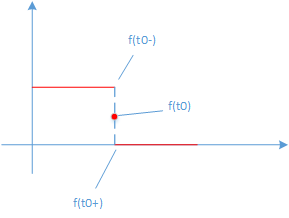
\includegraphics[width=0.4\textwidth]{assets/convergence.png}
		      \caption{跳变函数的收敛性}
	      \end{figure}
\end{enumerate}
\section{函数的内积}
\subsection{函数内积计算方法}
设有复变函数$f,g\in L^2([0,1])$,那么可以把$f,g$分别认为是Vector。求这两个Vector内积的方法为:
\begin{equation}
	(f,g)=\int_0^1\ f(t)\overline{g(t)}\ dt
\end{equation}
\begin{enumerate}
	\item $g(t)​$取共轭函数!!!!!
	\item 当$(f,g)=0$的时候,就可以说$f$与$g​$正交。
\end{enumerate}
\subsection{与Vector类比}
\begin{enumerate}
	\item 类比Vector的模:
	      $$
		      (f,f)=||f||^2=\int_0^1\ |f(t)|^2 \ dt
	      $$
	\item 当$f$与$g​$正交的时候,有函数形式的勾股定理:
	      $$
		      ||f+g||^2=||f||^2+||g||^2
	      $$
\end{enumerate}
\section{傅立叶级数与矩阵}
\subsection{空间内的Orthogonal Basis}
空间内一组标准正交向量:$q_1,q_2,\cdots ,q_n$。空间内任意向量$\mathbf{v}$有:
\begin{align*}
	v & =x_1\cdot q_1+x_2\cdot q_2+\cdots+x_n\cdot q_n=Q\cdot x \\
	x & =Q^{-1}\cdot v                                          \\
\end{align*}

因为$Q$为正交矩阵,所以$Q^T=Q^{-1}$,所以$x=Q^T\cdot v$。

因为$q_i$为标准Orthogonal Basis,所以$q_i^T\cdot q_j=0$。

所以$x_i=q_i^T\cdot v$。Vector与标准Orthogonal Basis的点乘,求得各分量。
\subsection{Orthogonal Basis}
\subsubsection{三角函数的Orthogonal Basis}
正弦余弦函数一定正交:
$$
	\int_0^{\frac{2\cdot \pi}{n}}\ \cos(n\cdot x)\sin(n\cdot x)=0
$$

相同频率的正弦函数不正交:
$$
	\int_0^{\frac{2\cdot \pi}{n}}\ \sin(n\cdot x)\sin(n\cdot x)=1
$$

相同频率的余弦函数不正交:
$$
	\int_0^{\frac{2\cdot \pi}{n}}\ \cos(n\cdot x)\cos(n\cdot x)=1
$$

由此性质,我们可以将$\sin(2\cdot \pi\cdot m \cdot t)$和$\cos(2\cdot \pi\cdot m \cdot t)$看作傅立叶级数上的Orthogonal Basis,來求解傅立叶系数。
\subsubsection{复指函数的Orthogonal Basis}
\begin{align*}
	  & (e^{2\cdot \pi\cdot i\cdot m\cdot t},e^{2\cdot \pi\cdot i\cdot n\cdot t})                      \\
	= & \int_0^1 \ e^{2\cdot \pi\cdot i\cdot m\cdot t}\cdot e^{2\cdot \pi\cdot i\cdot (-n)\cdot t}\ dt \\
	= & \int_0^1 \ e^{e^{2\cdot \pi\cdot i\cdot (m-n)\cdot t}}\ dt                                     \\
	= & \rsx{\frac{e^{2\cdot \pi\cdot i\cdot (m-n)\cdot t}}{2\cdot \pi \cdot i \cdot(m-n)}}_0^1
\end{align*}

展开$e^{2\cdot \pi\cdot i\cdot (m-n)\cdot t}$:
\begin{align*}
	  & e^{2\cdot \pi\cdot i\cdot (m-n)\cdot t}                                       \\
	= & \cos(2\cdot \pi \cdot t\cdot(m-n))+i \cdot \sin(2\cdot \pi \cdot t\cdot(m-n))
\end{align*}

因为$m,n\in \mathbb{Z}$,所以$m-n\in \mathbb{Z}$;所以$\cos(2\cdot \pi \cdot t\cdot(m-n))=1$;所以$\sin(2\cdot \pi \cdot t\cdot(m-n))=0$;所以$e^{2\cdot \pi\cdot i\cdot (m-n)\cdot t}-e^0=0$。

因此$e^{2\cdot \pi i\cdot k \cdot t}$被称为傅立叶变换中的Orthogonal Basis。
$$
	\begin{cases}
		(e^{2\cdot \pi\cdot i\cdot m\cdot t},e^{2\cdot \pi\cdot i\cdot m\cdot t}) & =1 \\
		(e^{2\cdot \pi\cdot i\cdot m\cdot t},e^{2\cdot \pi\cdot i\cdot n\cdot t}) & =0
	\end{cases}
$$
\subsection{求解傅立叶系数}
\subsubsection{三角函数形}
$f(t)$的三角函数表达式如下:

$$f(t)=\sum\limits_{k=1}^n\ [a_k\cdot \sin(2\cdot\pi\cdot k\cdot t) +b_k\cdot \cos(2\cdot \pi\cdot k\cdot t)]$$

将$f(t)$分别与$\sin(2\cdot \pi\cdot m \cdot t)$和$\cos(2\cdot \pi\cdot m \cdot t)$做内积,可以得到$a_m$和$b_m$:
\begin{align*}
	  & \int_0^1\ f(x)\cdot \sin(2\cdot \pi\cdot m \cdot t)\ dt            \\
	= & \int_0^1\ a_m\cdot \sin^2(2\cdot \pi\cdot m \cdot t)\ dt           \\
	= & \int_0^1\ a_m\cdot \frac{1-\cos(4\cdot \pi\cdot m \cdot t)}{2}\ dt \\
	= & \frac{a_m}{2}                                                      \\
\end{align*}
因此:
$$
	a_m=\frac{\int_0^1\ f(x)\cdot \sin(2\cdot \pi\cdot m \cdot t)\ dt}{\frac{1}{2}}
$$
同理:
$$
	b_m=\frac{\int_0^1\ f(x)\cdot \cos(2\cdot \pi\cdot m \cdot t)\ dt}{\frac{1}{2}}
$$
我们再来看看$c_m$:
\begin{align*}
	  & c_m                                                           \\
	= & \int_0^1 \ e^{-2\cdot \pi\cdot i\cdot m\cdot t}\cdot f(t)\ dt \\
	= & \int_0^1 \ [\cos(-2\cdot \pi\cdot i\cdot m\cdot t)            \\
	+ & i\cdot \sin(-2\cdot \pi\cdot i\cdot m\cdot t)\cdot f(t)]\ dt  \\
	= & \int_0^1 \ [\cos(2\cdot \pi\cdot i\cdot m\cdot t)             \\
	- & i\cdot \sin(2\cdot \pi\cdot i\cdot m\cdot t)\cdot f(t)]\ dt   \\
	= & \frac{b_m-i\cdot a_m}{2}
\end{align*}
与前面得到的结论一致。
\subsubsection{复指函数形}
如果$\mathbf{v}$是单位Vector,那么$(\mathbf{u},\mathbf{v})$是$\mathbf{u}$在$\mathbf{v}$上的投影。

类比到傅立叶级数:
\begin{align*}
	  & \hat{f}(k)                                                    \\                                          \\
	= & \int_0^1 \ f(t)\cdot e^{-2\cdot \pi\cdot i\cdot k\cdot t}\ dt \\
	= & (f(t),e^{2\cdot \pi\cdot i\cdot k\cdot t})
\end{align*}

因此傅立叶系数\ $\hat{f}(k)$是原函数$f(t)$在$e^{-2\cdot \pi\cdot i\cdot k\cdot t}$上的投影。

几何上的分量:
$$
	\mathbf{a}_{\mathbf{v}}=(\mathbf{a},\mathbf{v})\cdot \mathbf{v}
$$
\begin{enumerate}
	\item 先通过内积得到投影;
	\item 然后用投影乘上代表Vector方向的Orthogonal Basis得到该方向上的分量。
\end{enumerate}

类比到傅立叶级数:
\begin{align*}
	  & f(t)                                                                                                             \\
	= & \sum\limits_{k=-\infty}^\infty \ \hat{f}(t)\cdot e^{2\cdot \pi\cdot i\cdot k\cdot t}                             \\
	= & \sum\limits_{k=-\infty}^\infty\ (f,e^{2\cdot \pi\cdot i\cdot k\cdot t})\cdot e^{2\cdot \pi\cdot i\cdot k\cdot t}
\end{align*}

\begin{enumerate}
	\item 函数进行傅立叶级数后的每一项,都是函数在不同的Orthogonal Basis$e^{2\cdot \pi\cdot i\cdot k\cdot t}$上的分量。
	\item 反过来,这些分量相加构成完整的原始函数。
\end{enumerate}

下面补充Rayleigh's Identity。几何上,因为$\mathbf{c}^2=\mathbf{a}^2+\mathbf{b}^2$,所以$(\mathbf{a},\mathbf{b})=0$。类比到傅立叶级数,帕塞瓦尔定理的定义如下:
$$
	\int_0^1\ |f(t)|^2\ dt=\sum\limits_{k=-\infty}^{\infty}\ |\hat{f}(x)|^2
$$

傅立叶变换后的项互为正交项,正交项内积为$0$。
\section{卷积}
It is 卷积 in time, multiplication in 频率.

一般来说,频域的运算会比时域简单许多,因为频域只需执行相乘运算。
\subsection{定义}
设$f(t)$、$g(t)$是$\mathbb{R}$上两个可积函数,作积分:
$$
	\int_{-\infty}^\infty\ f(\tau)\cdot g(t-\tau)\ d\tau
$$
可以证明,关于几乎所有的 $x\in (-\infty ,\infty )$,上述积分是存在的。这样,随着$x$的不同取值,这个积分就定义了一个新函数$h(x)$,称为函数$f$与$g$的卷积,记为:
$$
	h(x)=(f*g)(t)=\int_{-\infty}^{\infty}\ f(r)\cdot g(t-r)\ dr
$$
\subsection{卷积与偏微分方程}
偏微分方程的解经常以卷积的形式出现。卷积的一方是特解,另一方是给定的初始数据下的初始条件。
\subsection{图解卷积}
\begin{figure}[H]
	\centering
	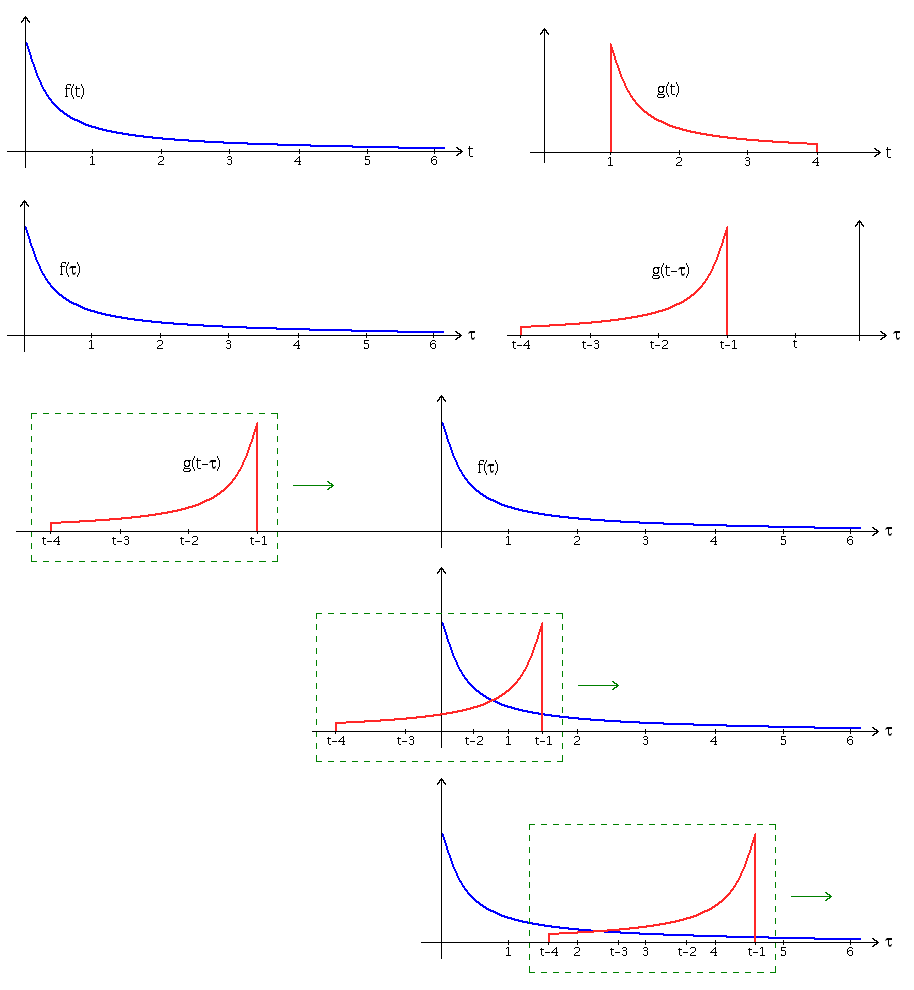
\includegraphics[width=0.4\textwidth]{assets/Convolution.png}
	\caption{图解卷积}
\end{figure}

\begin{enumerate}
	\item 已知两函数$f(t)$和$g(t)$。上图第一行分别为$f(t)$和$g(t)$。
	\item 首先将两个函数都用$\tau$来表示,从而得到$f(\tau)$和$g(\tau)$。将函数$g(\tau)$向右移动t个单位,得到函数$g(\tau-t)$的图像。将$g(\tau-t)$翻转至纵轴另一侧,得到$g(t-\tau)$的图像。上图第二行两图分别为$f(\tau)$和$g(t-\tau)$。
	\item 由于$\tau$是时间变量,当时间变量(以下简称“时移”)取不同值时,$g(t-\tau)$能沿着$\tau$轴“滑动”。右图第三四五行可理解为“滑动”。
	\item 让$\tau$从$-∞$滑动到$+∞$。两函数交会时,计算交会范围中两函数乘积的积分值。换句话说,我们是在计算一个滑动的的加权总和。也就是使用$g(t-\tau )$当做加权函数,来对$f(\tau)$取加权值。
	\item 最后得到的波形(未包含在此图中)就是$f$和$g$的卷积。如果$f(t)$是一个单位脉冲,我们得到的乘积就是$g(t)$本身,称为冲激响应。
\end{enumerate}